\begin{frame}{Semana 1 (06/02/2024) - T1}
        \textbf{Trabajo}

        $$W_{12}=\int_{1}^{2}\vec{\boldsymbol{F}}\boldsymbol{\cdot} d\vec{\boldsymbol{s}}.$$
\end{frame}

\begin{frame}{Semana 1 (06/02/2024) - T1P1}

La masa del niño es $m$, la longitud
de las cadenas es $R$, y se empuja con una fuerza $F$ hasta que las cadenas forman un
ángulo $\theta_0$ con la vertical. La fuerza $F$ es horizontal, variable, comienza en cero y aumenta en forma gradual apenas lo suficiente para que el niño y el columpio se muevan lentamente y permanezcan casi en equilibrio.

¿Qué trabajo total realizan todas las
fuerzas sobre el niño? ¿Qué trabajo realiza la tensión en las cadenas? ¿Qué trabajo efectúa la fuerza $F$? (Ignore el peso
de las cadenas y el asiento).

\begin{figure}[H]
    \centering
    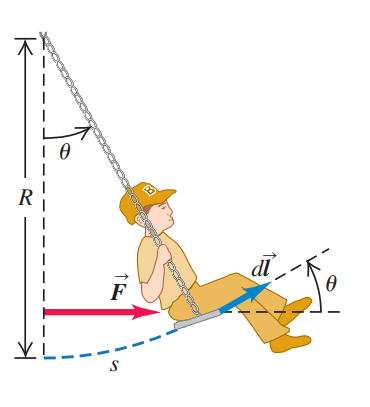
\includegraphics[width=0.3\textwidth]{figures/t1t1.png}
\end{figure}
    
\end{frame}

\begin{frame}{Semana 1 (06/02/2024) - T1}
    \textbf{Energía cinética}
    $$W_{12}=K_2-K_1=\frac{m}{2}\left(v_2^2-v_1^2\right).$$
    
    \textbf{Energía potencial}
    
    Si $W_{12}$ es independiente de la trayectoria:
    $$W_{12}=U_1-U_2,$$
    $$\vec{\boldsymbol{F}}=-\vec{\boldsymbol{\nabla}}U(\vec{\boldsymbol{r}}),$$
    $$\oint_1^2\vec{\boldsymbol{F}}\boldsymbol{\cdot} d\vec{\boldsymbol{s}}=0.$$
    
    \textbf{Conservación de la energía}
    $$K_1+U_1=K_2+U_2.$$
\end{frame}

\begin{frame}{Semana 1 (06/02/2024) - T1P2}

    \textbf{Atwood's Machine}

    \begin{figure}[H]
    \centering
    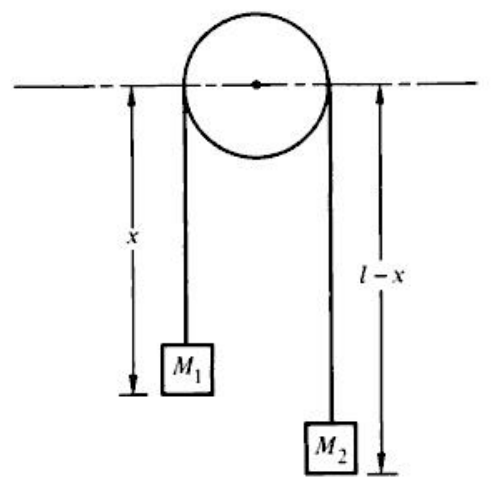
\includegraphics[width=0.5\textwidth]{figures/t1t2.png}
\end{figure}
    
\end{frame}

\begin{frame}{Semana 2 (13/02/2024) - T2P1}
        $X$ e $Y$ son dos esferas de metal sin carga sobre soportes aislantes y están en contacto entre sí. Una barra R cargada positivamente se acerca a $X$ como se muestra en la figura (a).
        
        La esfera $Y$ ahora se aleja de $X$, como en la figura (b).
        
        ¿Cuáles son los estados de carga finales de $X$ e $Y$?
        
        \begin{figure}
            \centering
            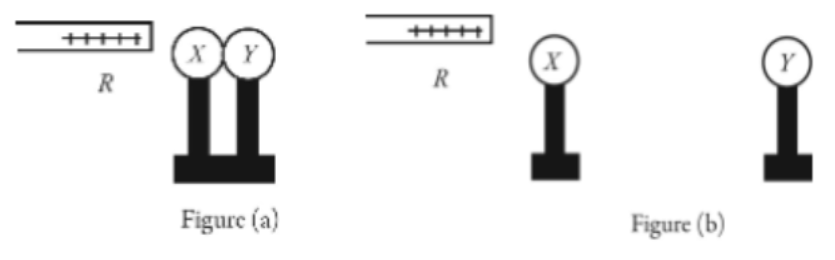
\includegraphics[scale=0.3]{figures/t2p1.png}
        \end{figure}
        
        \begin{columns}
        \column{0.5\textwidth}
        \begin{itemize}
            \item[A)] Tanto $X$ como $Y$ son neutros.
            \item[B)] $X$ es positivo e $Y$ es neutro.
            \item[C)] $X$ es neutro e $Y$ es positivo.
            \end{itemize}
        \column{0.5\textwidth}
        \begin{itemize}
            \item[D)] $X$ es negativo y $Y$ es positivo.
            \item[E)] Tanto $X$ como $Y$ son negativos.
        \end{itemize}
        \end{columns}
        
        
        
        \pause\bigskip\centering \textbf{Respuesta:} D.
\end{frame}

\begin{frame}{Semana 2 (13/02/2024) - T2P2}
    
    Una carga puntual positiva $Q$ está fija sobre una mesa horizontal muy grande sin fricción. Una segunda carga puntual positiva $q$ se libera desde el reposo cerca de la carga estacionaria y puede moverse libremente. ¿Qué enunciado describe mejor el movimiento de $q$ después de que se suelta?
    
    \begin{itemize}
    
    \item[A)]Su velocidad será máxima justo después de que se suelte.

    \item[B)] Su aceleración es cero justo después de que se suelta.
    
    \item[C)] A medida que se aleja más y más de $Q$, su aceleración seguirá aumentando.
    
    \item[D)] A medida que se aleja más y más de $Q$, su velocidad disminuirá.
    
    \item[E)] A medida que se aleja más y más de $Q$, su velocidad seguirá aumentando.
    \end{itemize}
    
    \pause\bigskip\centering\textbf{Respuesta:} E.
    
\end{frame}

\begin{frame}{Semana 2 (13/02/2024) - T2P3}
    
    Una bola de plástico muy pequeña cargada uniformemente está ubicada directamente encima de otra carga similar en un tubo de ensayo como se muestra en la figura. Las bolas están en equilibrio a una distancia $d$.
    
    \begin{columns}
    \column{0.5\textwidth}
     \begin{figure}
        \centering
        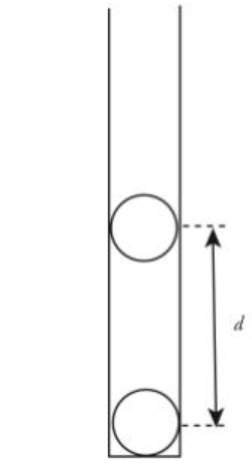
\includegraphics[scale=0.3]{figures/t2p3.png}
    \end{figure}
    
    \column{0.5\textwidth}

Si se duplica la carga de cada bola, la distancia entre las bolas en el tubo de ensayo sería
    
     \begin{itemize}
        \item[A)] $\sqrt{2}d$
        \item[B)] $2d$
        \item[C)] $4d$
        \item[D)] $8d$
    \end{itemize}
    
    \pause\bigskip\centering\textbf{Respuesta:} B.

    \end{columns}
    
\end{frame}

\begin{frame}{Semana 2 (13/02/2024) - T2P4}
    
    En la figura, $Q = 5.8$ nC. ¿Cuál es la magnitud de la fuerza el\'ectrica sobre la carga $Q$?
    
    \begin{figure}
        \centering
        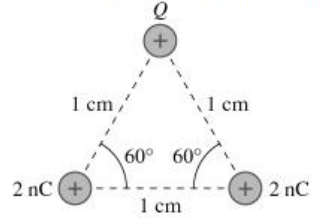
\includegraphics[scale=0.5]{figures/t2p4.png}
    \end{figure}
    
\end{frame}

\begin{frame}{Semana 2 (13/02/2024) - T2P5}
    Cuatro cargas puntuales negativas iguales están ubicadas en las esquinas de un cuadrado, sus posiciones en el plano $xy$ son $(1, 1)$, $(-1, 1)$, $(-1, -1)$ y $(1, -1)$. Si se posiciona una carga positiva en el punto $(1,0)$, determine la direcci\'on de la fuerza el\'ectrica que esta experimenta.
\end{frame}

\begin{frame}{Semana 2 (13/02/2024) - T2P6}
    
    Determine la magnitud y direcci\'on de la fuerza el\'ectrica que experimenta una carga puntual positiva $q$ ubicada en el punto $(L,d)$, debida a una barra delgada cargada homogéneamente con una carga $Q$ negativa y que est\'a sobre el eje $x$ en $0\leq x\leq L$.
    
\end{frame}

\begin{frame}{Semana 2 (13/02/2024) - T2P7}
    
    La figura muestra dos diminutas esferas de masa $m$ que est\'an suspendidas de dos hilos muy delgados de longitud $L$. Las esferas se repelen entre sí después de cargarse con la misma magnitud de carga $Q$ y cuelgan en reposo como se muestra en la figura. ¿Cuál es valor del ángulo $\theta$?
    
    \begin{figure}
        \centering
        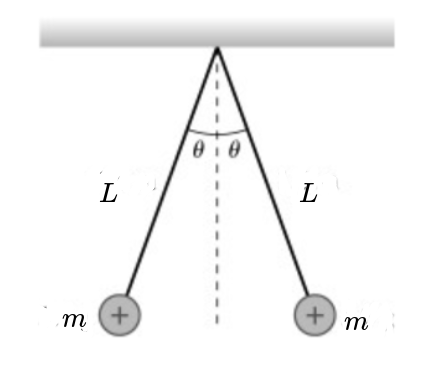
\includegraphics[scale=0.4]{figures/t2p7.png}
    \end{figure}
    
\end{frame}

\begin{frame}{Semana 2 (13/02/2024) - T2P8}
Considere cuatro cargas $q$ negativas fijas en los vértices de un cuadrado de lado $2L$.
Demuestre que si una carga $Q$ positiva de masa $m$ se libera a una pequeña distancia horizontal $\epsilon$ del centro del cuadrado, describirá un movimiento oscilatorio con frecuencia angular $$\omega\sim\frac{1}{L}\sqrt{k_e\frac{qQ}{mL}}.$$
\end{frame}

\begin{frame}{Semana 3 (20/02/2024) - T3P1}

    La figura muestra tres cargas eléctricas etiquetadas como $Q_1$, $Q_2$, $Q_3$ y algunas líneas de campo eléctrico en la región que rodea las cargas.
    
    \begin{figure}[H]
        \centering
        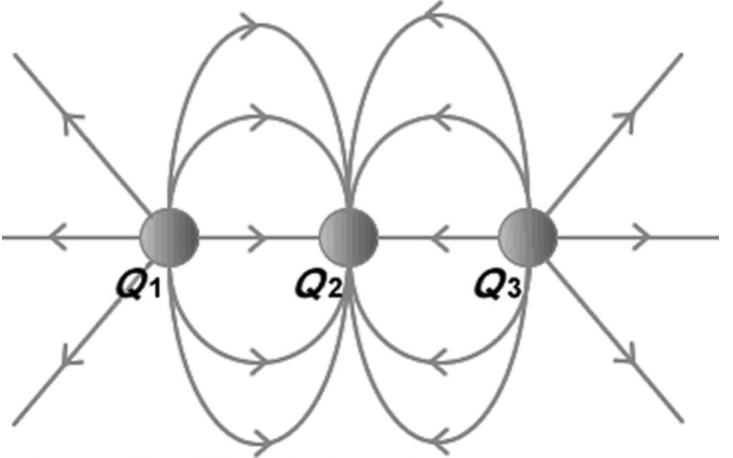
\includegraphics[scale=0.2]{figures/t3p1.png}
    \end{figure}
    
    ¿Cuáles son los signos de las tres cargas?
    
    \begin{columns}
    \column{0.5\textwidth}
    \begin{itemize}
        \item[A)] $Q_1$ es positivo, $Q_2$ es negativo y $Q_3$ es positivo.
        \item[B)] $Q_1$ es negativo, $Q_2$ es positivo y $Q_3$ es negativo.
    \end{itemize}
    \column{0.5\textwidth}
    \begin{itemize}
        \item[C)] $Q_1$ es positivo, $Q_2$ es positivo y $Q_3$ es negativo.
        \item[D)] Las tres cargas son negativas.
        \item[E)] Las tres cargas son positivas.
    \end{itemize}
    
    \end{columns}
    
    \pause\bigskip\centering\textbf{Respuesta:} A.
    
\end{frame}

\begin{frame}{Semana 3 (20/02/2024) - T3P2}

    Un electrón se mueve inicialmente hacia la derecha cuando entra en un campo eléctrico uniforme dirigido hacia arriba.
    
    \begin{figure}
        \centering
        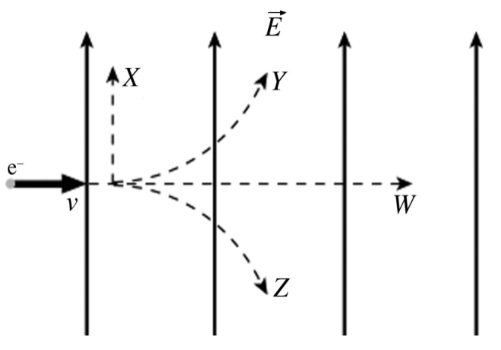
\includegraphics[scale=0.3]{figures/t3p2.png}
    \end{figure}
    
    ¿Cuál de las trayectorias mostradas seguirá el electrón?
    
    \begin{columns}
    \column{0.2\textwidth}
    
    \begin{itemize}
        \item[A)] W.
        \item[B)] X.
    \end{itemize}
    
    \column{0.2\textwidth}
    
    \begin{itemize}
        \item[C)] Y.
        \item[D)] Z.
    \end{itemize}
    
    \column{0.2\textwidth}
    \pause\centering\textbf{Respuesta:} D.
    \end{columns}
    
\end{frame}

\begin{frame}{Semana 3 (20/02/2024) - T3P3}

    Un dipolo eléctrico inicialmente estacionario de momento dipolar $\Vec{p}=\left(5.0\times10^{-10}\text{ C}\cdot\text{m }\right)\hat{\imath},$ es colocado en un campo eléctrico $\vec{E}=\left( 2.00\times10^6\text{ N/C} \right)\left(\hat{\imath}+\hat{\jmath}\right)$ ¿Cuál es la magnitud del torque máximo que el campo eléctrico ejerce sobre el dipolo?
    
\end{frame}

\begin{frame}{Semana 3 (20/02/2024) - T3P4}

    Un dipolo eléctrico consta de cargas $\pm Q$ separadas una distancia $d$. Está colocado en un campo eléctrico vertical de magnitud $E$ orientado como se muestra en la figura.
    
    \begin{columns}
    \column{0.5\textwidth}
    
    \begin{figure}
        \centering
        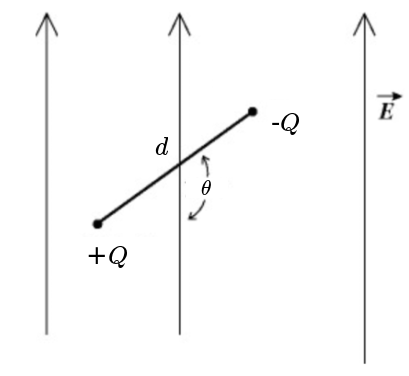
\includegraphics[scale=0.35]{figures/t3p4.png}
    \end{figure}
    
    \column{0.5\textwidth}
    
    La magnitud del torque neto que este campo ejerce sobre el dipolo est\'a dada por
    
    \begin{itemize}
        \item[A)] $QEd\sin\theta$.
        \item[B)] $\frac{QE}{2}d\cos\theta$.
        \item[C)] $QEd\cos\theta$.
        \item[D)] $\frac{QE}{2}d\sin\theta$.
    \end{itemize}
    
    \pause\bigskip\centering\textbf{Respuesta:} A.
    
    \end{columns}
    
\end{frame}

\begin{frame}{Semana 3 (20/02/2024) - T3P5}
    
    Determine la magnitud y direcci\'on de la fuerza el\'ectrica que experimenta una carga puntual positiva $q$ ubicada en el punto $(L,d)$, debida a una barra delgada cargada homogéneamente con una carga $Q$ negativa y que est\'a sobre el eje $x$ en $0\leq x\leq L$.
    
\end{frame}

\begin{frame}{}

    \textbf{Pasos para solucionar un problema con diferenciales}

    \begin{enumerate}
        \item Analice si el sistema verifica simetrías que permiten despreciar o cancelar fuerzas en una o varias direcciones. 
        \item Escoja un elemento diferencial (longitud, área o volumen) en función de una de las variables del sistema coordenado ($x$, $y$, $\theta$, $r$, etc):
        \begin{equation*}
            dq = \lambda dl,\, \sigma dA\, \text{ó}\, \rho dV,
        \end{equation*}

        donde se definen las densidades lineal, superficial y volumétrica de carga como:
        \begin{equation*}
            \lambda = \frac{q}{l},\, \sigma = \frac{q}{A}\, \text{y}\, \rho = \frac{q}{V}
        \end{equation*}
        \item Defina el vector de posición $\vec{r}$ en función de la misma variable que escogió para el elemento diferencial.
        \item Integre sobre todo recorrido de la variable en cuestión.
    \end{enumerate}
    
\end{frame}

\begin{frame}{}
    \begin{enumerate}
        \setcounter{enumi}{4}
        \item En caso de ser posible, considere las siguientes aproximaciones
        \begin{equation*}
        \begin{aligned}
            (1+x^2)^{-1/2}&=\sum_{k=0}^\infty (-1)^k\frac{(2k-1)!!}{(2k)!!}x^{2k},\\
            (1+x^2)^{-3/2}&=\sum_{k=0}^\infty (-1)^k\frac{(2k+1)!!}{(2k)!!}x^{2k},
        \end{aligned}
        \end{equation*}
        donde se define el doble factorial como 
        \begin{equation*}
            \begin{aligned}
            (2k-1)!!&=1\cdot3\cdot5\cdot\dots\cdot(2k-3)(2k-1)=\frac{(2k)!}{2^kk!},\\
            (2k)!!&=2\cdot4\cdot6\cdot\dots\cdot(2k-2)(2k)=2^kk!.
            \end{aligned}
        \end{equation*}
        En otro caso, utilice sustitución trigonométrica de ser posible.
    \end{enumerate}
\end{frame}

\begin{frame}{Semana 3 (20/02/2024) - T3P6}

Un semicírculo de radio $a$ se encuentra en los cuadrantes primero y segundo, y con el centro de curvatura en el origen. La carga positiva $+Q$ está distribuida de manera uniforme alrededor de la mitad izquierda del semicírculo, y la carga negativa $-Q$ está distribuida de manera uniforme
alrededor de la mitad derecha del semicírculo como lo muestra la figura.

\begin{figure}
    \centering
    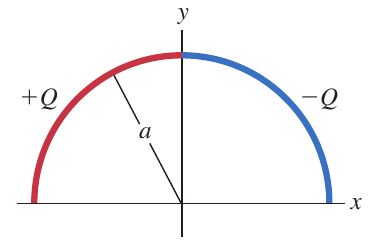
\includegraphics[scale=0.3]{figures/t3p6.png}
\end{figure}

¿Cuál es la magnitud y dirección del campo eléctrico neto en el origen generado por esta distribución de carga?

Calcule ahora el campo en un punto que esté a una distancia $h$ del origen, fuera del plano que contiene las distribuciones.
    
\end{frame}

\begin{frame}{Semana 3 (20/02/2024) - T3P7 (Bonus)}
    Considere dos alambres delgados que est\'an sobre el eje $x$. El primero se encuentra en $-d/2-L<x<-d/2$ y el segundo en $d/2<x<d/2+L$. Cada uno tiene longitud $L$ y posee carga positiva $Q$ distribuida uniformemente.
    
    \begin{itemize}
        \item[a)] Determine el campo el\'ectrico que el primer alambre genera sobre el eje $x$ positivo.
        \item[b)] Demuestre que la magnitud de la fuerza el\'ectrica que un alambre ejerce sobre el otro est\'a dada por
        
        \begin{equation}
            F=\frac{1}{4\pi\epsilon_0}\left(\frac{Q}{L}\right)^2\ln\left[\frac{\left(d+L\right)^2}{d(d+2L)}\right]
        \end{equation}
        
        \item[c)] Demuestre que si $L<<d$, entonces
        
        \begin{equation}
            F=\frac{1}{4\pi\epsilon_0}\left(\frac{Q}{d}\right)^2.
        \end{equation}
        
    \end{itemize}

\end{frame}

\begin{frame}{Semana 3 (20/02/2024) - Q1}
    
    En cada vértice de un cuadrado hay una partícula de carga $q$. En el centro del cuadrado está fija una carga puntiforme de signo contrario, de valor $Q$, ¿Cuál debe ser el valor de $Q$ para que la fuerza total sobre cada una de las cuatro partículas sea nula? Considere que la única fuerza actuante sobre el sistema es eléctrica.

\end{frame}

\begin{frame}{Semana 4 (27/02/2024) - T4}
    
    \begin{figure}
        \centering        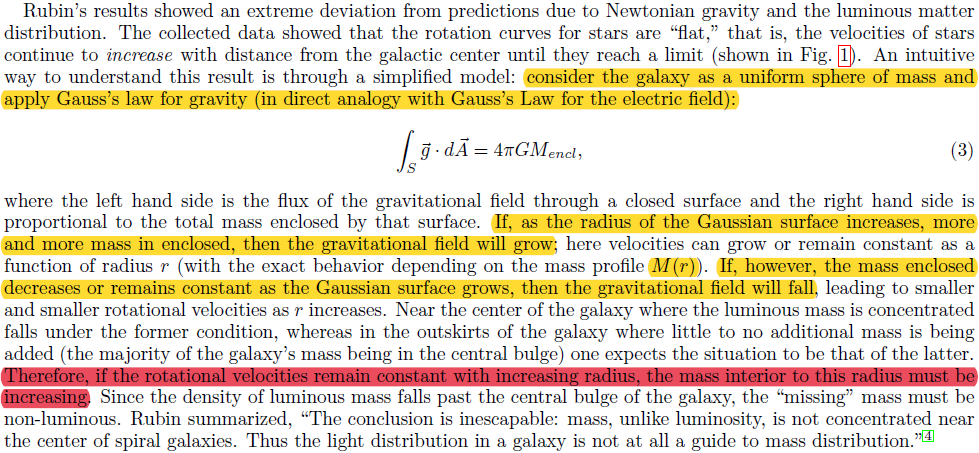
\includegraphics[width=1\textwidth,height=0.7\textwidth]{figures/t4t1.png}
    \end{figure}

\end{frame}

\begin{frame}{Semana 4 (27/02/2024) - T4P1}
    
    La figura muestra cuatro superficies gaussianas que rodean una distribución de cargas puntuales.
    
    \begin{figure}
        \centering
        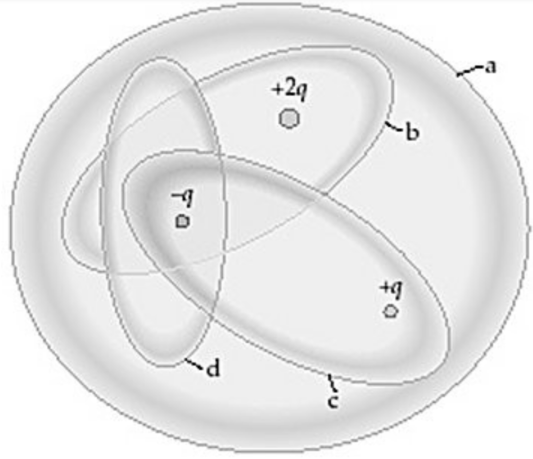
\includegraphics[scale=0.25]{figures/t4p1.png}
    \end{figure}
    
    \begin{itemize}
        \item[a)] ¿Qué superficies gaussianas tienen un flujo eléctrico de $+q/\epsilon_0$ a través de ellas? 
        \pause \textbf{Respuesta:} b
        \pause \item[b)] ¿Qué superficies gaussianas no tienen flujo eléctrico a través de ellas? 
        \pause \textbf{Respuesta:} c
    \end{itemize}
    
\end{frame}

\begin{frame}{Semana 4 (27/02/2024) - T4P2}
    
    ¿Cuáles de las siguientes afirmaciones sobre la ley de Gauss son correctas? (Puede haber más de una opción correcta).
    
    \begin{itemize}
        \item[A)] La ley de Gauss es válida solo para distribuciones de carga simétricas, como esferas y cilindros.

        \item[B)] Si no hay carga dentro de una superficie gaussiana, el campo eléctrico debe ser cero en los puntos de esa superficie.
        
        \item[C)] Solo la carga encerrada dentro de una superficie gaussiana puede producir un campo eléctrico en puntos de esa superficie.
        
        \item[D)] Si una superficie gaussiana está completamente dentro de un conductor electrostático, el campo eléctrico siempre debe ser cero en todos los puntos de esa superficie.
        
        \item[E)] El flujo eléctrico que pasa a través de una superficie gaussiana depende únicamente de la cantidad de carga dentro de esa superficie, no de su tamaño o forma.
    \end{itemize}
    
    \pause\bigskip\centering\textbf{Respuesta:} D y E.
    
\end{frame}

\begin{frame}{Semana 4 (27/02/2024) - T4P3}
    \begin{columns}
    \column{1.1\textwidth}
    \footnotesize
    
    El gráfico de la figura muestra la intensidad del campo eléctrico en función de la distancia desde el centro de un par de esferas concéntricas uniformemente cargadas. 
    ¿Cuál de las siguientes situaciones podría representar plausiblemente el gráfico? (Puede haber más de una opción correcta).
    \vspace{-2em}
    \begin{figure}
        \centering
        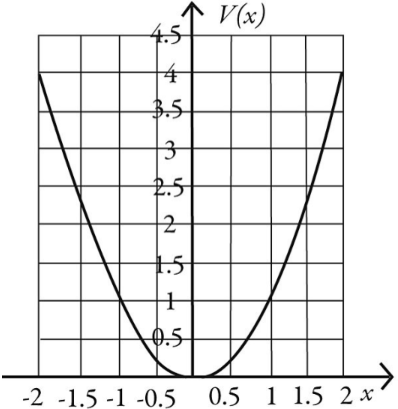
\includegraphics[scale=0.2]{figures/t4p3.png}
    \end{figure}
    \vspace{-2em}
    \begin{itemize}
        \item[A)] Una esfera conductora cargada positivamente dentro de otra esfera conductora cargada positivamente.
        \item[B)] Una esfera conductora cargada positivamente dentro de una esfera conductora sin carga.
        \item[C)] Una esfera sólida no conductora, uniformemente cargada en todo su volumen, dentro de una esfera conductora cargada positivamente.
        \item[D)] Una capa esférica de pared delgada no conductora cargada positivamente dentro de una esfera conductora cargada positivamente.
        \item[E)] Una capa esférica de pared delgada no conductora cargada positivamente dentro de otra capa esférica de pared delgada no conductora cargada positivamente.
    \end{itemize}
    \pause \centering\textbf{Respuesta:} A, B y D.
    
    \end{columns}

\end{frame}

\begin{frame}{Semana 4 (27/02/2024) - T4P4}
    
    A una distancia $d$ de una línea de carga uniforme muy larga (esencialmente infinita), la intensidad del campo eléctrico es $E$. ¿A qué distancia de la línea la intensidad del campo será $2E$?
    
    \begin{columns}
    \column{0.4\textwidth}
    \begin{itemize}
        \item[A)] $2d$
        \item[B)] $\sqrt{2}d$
        \item[C)] $d/\sqrt{2}$
        \item[D)] $d/2$
        \item[E)] $d/4$
    \end{itemize}
    \column{0.5\textwidth}
    \pause\centering\textbf{Respuesta:} D.
    \end{columns}
    
\end{frame}

\begin{frame}{Semana 4 (27/02/2024) - T4P5}
    
    Una capa esférica no conductora de radio interior $R_1$ y radio exterior $R_2$ contiene una densidad de carga volum\'etrica uniforme $\rho$ en toda la capa. Use la ley de Gauss para derivar una ecuación para la magnitud del campo eléctrico a las siguientes distancias radiales $r$ desde el centro de la esfera. Exprese las respuestas deben estar en términos de $\rho$, $R_1$, $R_2$, $r$, $\epsilon_0$ y $\pi$.
    
    \begin{itemize}
        \item[a)] $r<R_1$
        \item[b)] $R_1<r<R_2$
        \item[c)] $r>R_2$
    \end{itemize}
    
    \pause\textbf{Respuestas:} 
    \begin{columns}
    \column{0.2\textwidth}
    \begin{itemize}
        \item[a)] $E=0$.
    \end{itemize}
    \column{0.4\textwidth}
    \begin{itemize}
        \item[b)] $E=\frac{\rho}{3\epsilon_0 r^2}\left(r^3-R_1^3\right)$.
    \end{itemize}
    \column{0.4\textwidth}
    \begin{itemize}
        \item[c)] $E=\frac{\rho}{3\epsilon_0 r^2}\left(R_2^3-R_1^3\right)$.
    \end{itemize}
    \end{columns}
    
\end{frame}

\begin{frame}{Semana 4 (27/02/2024) - T4P6}
    
    Considere una placa infinita no conductora de espesor $a$, cargada uniformemente con una densidad volum\'etrica de carga $\rho$. Determine la magnitud del campo el\'ectrico en
    
    \begin{itemize}
        \item[a)] Un punto fuera de la placa.
        \item[b)] Un punto en el interior de la placa.
    \end{itemize}
    
\end{frame}

\begin{frame}{Semana 4 (27/02/2024) - T4P7}
    
    Considere dos placas metálicas paralelas muy próximas entre sí y con cargas opuestas. Las placas son cuadradas con lados de longitud $L$ y llevan cargas $Q$ y $-Q$ en sus superficies enfrentadas. ¿Cuál es la magnitud del campo eléctrico en la región entre las placas?
    
    \begin{itemize}
        \item[A)] $E = \frac{Q}{\epsilon_0L^2}$
        \item[B)] $E = \frac{2Q}{\epsilon_0L^2}$.
        \item[C)] $E=0$.
        \item[D)] $E = \frac{4Q}{\epsilon_0L^2}$.
        \item[E)] $E = \frac{Q}{2\epsilon_0L^2}$.
    \end{itemize}
    
    \pause\bigskip\centering\textbf{Respuesta:} A.
    
\end{frame}

\begin{frame}{Semana 4 (27/02/2024) - T4P8}
  
  Dos alambres no conductores de longitud $L=\infty$ cada uno, forman un ángulo recto. Un segmento tiene una carga neta de $-Q$, distribuida de modo uniforme por toda su longitud; el otro segmento tiene tiene una carga neta de $+Q$, distribuida de modo uniforme por toda su longitud, como se ilustra en la figura.
    
    \begin{columns}
    
    \column{0.5\textwidth}
    
    \begin{figure}
        \centering
        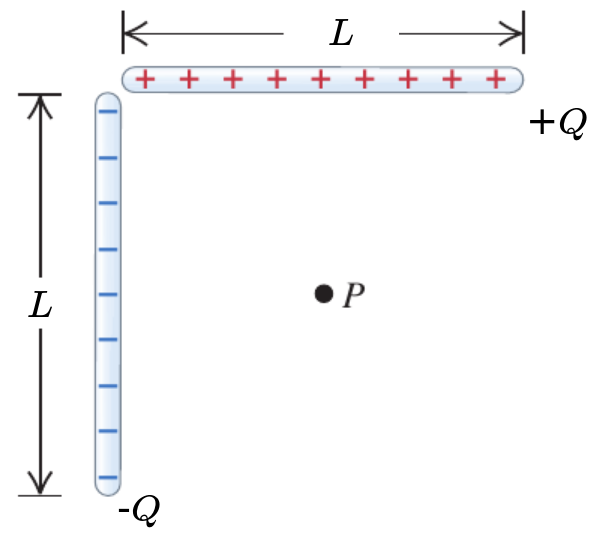
\includegraphics[scale=0.25]{figures/t4p8.png}
    \end{figure}
    
    \column{0.5\textwidth}
    
    Aplique la ley de gauss para determinar la magnitud del campo el\'ectrico que produce cada alambre en el punto $P$, que dista $d$ de cada alambre. Luego, deduzca las direcciones de cada campo y determine el campo el\'ectrico total en $P$.
    
    \end{columns}
    
\end{frame}

\begin{frame}{Semana 4 (27/02/2024) - T4P9 (Desafío)}
  
  A ring with radius $R$ has uniform positive charge density $\lambda$. A particle with positive charge $q$ and mass $m$ is initially located at the center of the ring and is then given a tiny kick. If it is constrained to move in the plane of the ring, show that it undergoes simple harmonic motion (for small oscillations), and find the frequency.
    
\end{frame}

\begin{frame}{Semana 5 (05/03/2024) - T5P1}
    
    If the electric field is zero everywhere inside a region of space, the potential must also be zero in that region.
    
    \begin{itemize}
        \item[A)] True.
        \item[B)] False.
    \end{itemize}
    
    
    When the electric field is zero at a point, the potential must also be zero there.
    
    \begin{itemize}
        \item[A)] True.
        \item[B)] False.
    \end{itemize}
    
    If the electrical potential in a region is constant, the electric field must be zero everywhere in that region.
    
    \begin{itemize}
        \item[A)] True.
        \item[B)] False.
    \end{itemize}
    
    f the electric potential at a point in space is zero, then the electric field at that point must also be zero.
    
    \begin{itemize}
        \item[A)] True.
        \item[B)] False.
    \end{itemize}
    
\end{frame}

\begin{frame}{Semana 5 (05/03/2024) - T5P1}
    
    If the electric field is zero everywhere inside a region of space, the potential must also be zero in that region.
    
    \begin{itemize}
        \item[A)] True.
        \item[B)] False. $\leftarrow$ \textbf{Answer}
    \end{itemize}
    
    
    When the electric field is zero at a point, the potential must also be zero there.
    
    \begin{itemize}
        \item[A)] True.
        \item[B)] False. $\leftarrow$ \textbf{Answer}
    \end{itemize}
    
    If the electric potential in a region is constant, the electric field must be zero everywhere in that region.
    
    \begin{itemize}
        \item[A)] True. $\leftarrow$ \textbf{Answer}
        \item[B)] False.
    \end{itemize}
    
    If the electric potential at a point in space is zero, then the electric field at that point must also be zero.
    
    \begin{itemize}
        \item[A)] True.
        \item[B)] False. $\leftarrow$ \textbf{Answer}
    \end{itemize}
    
\end{frame}

\begin{frame}{Semana 5 (05/03/2024) - T5P2}
    Una esfera metálica de 5 cm de radio está cargada de tal manera que el potencial el\'ectrico en su superficie es de 100 V (relativo al infinito). ¿Cuál de las siguientes gráficas muestra correctamente el potencial el\'ectrico en función de la distancia desde el centro de la esfera?
    
    \vspace{-2em}
    
    \begin{figure}
        \centering
        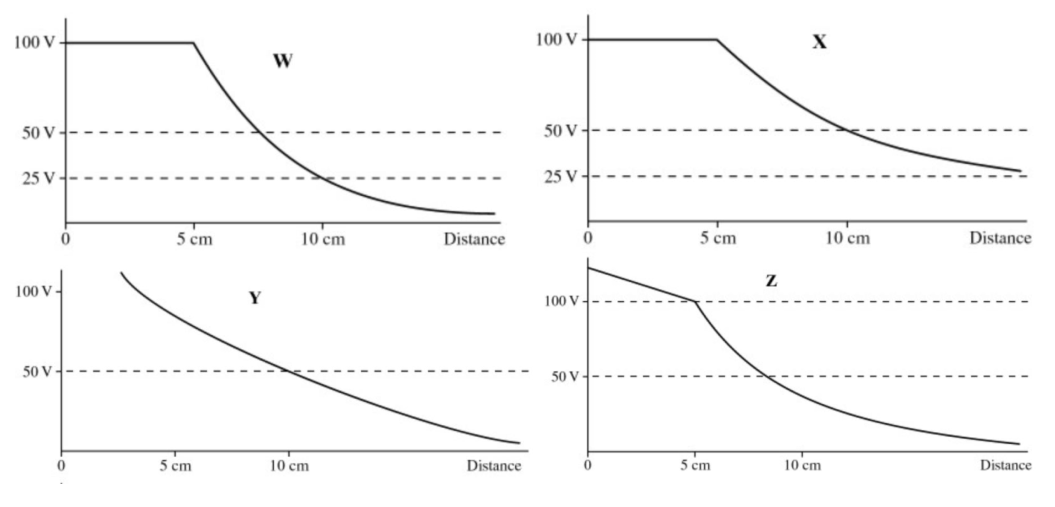
\includegraphics[scale=0.3]{figures/t5p2.png}
    \end{figure}
    
    \pause \begin{center}
        \textbf{Respuesta:} X.
    \end{center}
    
\end{frame}



\begin{frame}{Semana 5 (05/03/2024) - T5P3}
    
    \vspace{-1em}
    
    \begin{columns}
    \column{0.5\textwidth}
    El gráfico de la figura muestra la variación del potencial eléctrico $V(x)$ en función de la posición $x$.
    \column{0.4\textwidth}
    \begin{figure}
        \centering
        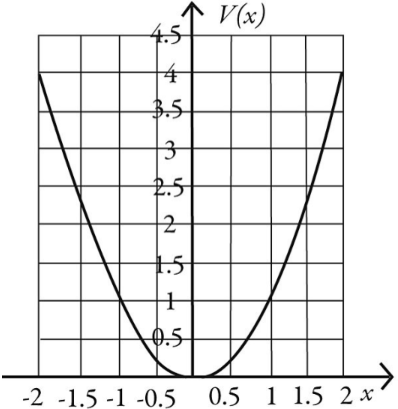
\includegraphics[scale=0.3]{figures/t5p3.png}
    \end{figure}
    \end{columns}
    
    \vspace{1em}
    
    ¿Cuál de las siguientes opciones describe correctamente la orientación de la componente $x$ del campo eléctrico a lo largo del eje $x$?
    
    \begin{itemize}
        \item[A)] $E_x$ es positivo desde $x = -2$ hasta $x = 2$.

        \item[B)] $E_x$ es positivo desde $x = -2$ hasta $x = 0$, y negativo desde $x = 0$ hasta $x = 2$.
        
        \item[C)] $E_x$ es negativo de $x = -2$ a $x = 0$, y positivo de $x = 0$ a $x = 2$.
        
        \item[D)] $E_x$ es negativo desde $x = -2$ hasta $x = 2$.
    \end{itemize}
    
    \pause \begin{center}
        \textbf{Respuesta:} B.
    \end{center}
    
\end{frame}

\begin{frame}{Semana 5 (05/03/2024) - T5P4}
    Una carga puntual de $+$4.0 $\mu$C y una carga puntual de $-$4.0 $\mu$C se colocan como se muestra en la figura. ¿Cuál es la diferencia de potencial, $V_A-V_B$, entre los puntos $A$ y $B$?
    
    \begin{figure}
        \centering
        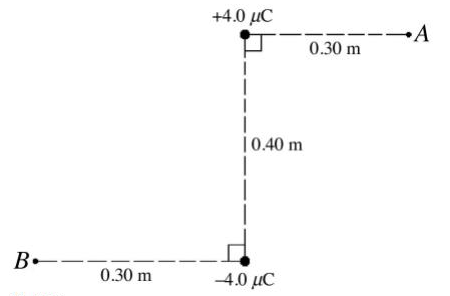
\includegraphics[scale=0.5]{figures/t5p4.png}
    \end{figure}
    
\end{frame}

\begin{frame}{Semana 5 (05/03/2024) - T5P5}
    The figure shows two arcs of a circle on which charges $+Q$ and $-Q$ have been spread uniformly. What is the value of the electric potential at the center of the circle?
    
    \begin{figure}
        \centering
        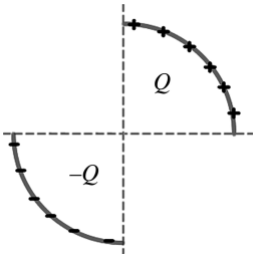
\includegraphics[scale=0.5]{figures/t5p5.png}
    \end{figure}
    
\end{frame}

\begin{frame}{Semana 5 (05/03/2024) - T5P6}

    Un positrón tiene una masa de $9.11\times10^{-31}$ kg y una carga $q_0 = +e = 1.60 \times 10^{-19}$ C. Suponga que un
positrón se mueve en la vecindad de una partícula $\alpha$ (alfa) cuya carga
es $q = +2e = 3.20 \times 10^{–19}$ C y con masa $6.64 \times 10^{-27}$ kg. La partícula $\alpha$
tiene una masa $7\,000$ veces mayor que la del positrón, por lo que se
supondrá que está en reposo. Cuando el positrón está a $1.00 \times 10^{-10}$ m
de la partícula $\alpha$, se aleja de esta con una rapidez de $3.00 \times 10^6$ m/s.

\begin{itemize}
    \item[a)] ¿Cuál es la rapidez del positrón cuando las dos partículas están separadas una distancia de $2.00 \times 10^{-10}$ m?
    \item[b)] ¿Cuál es la rapidez del
positrón cuando está muy alejado de la partícula alfa?
    \item[c)] Suponga
que las condiciones iniciales son las mismas, pero la partícula que se
mueve es un electrón (con la misma masa que el positrón, pero con
carga $q_0 = -e$). Describa el movimiento subsiguiente.
\end{itemize}
    
\end{frame}

\begin{frame}{Semana 5 (05/03/2024) - T5P7}
    Dos cargas puntuales de $+$1.0 $\mu$C y $-$2.0 $\mu$C están ubicadas a 0.50 m de distancia. ¿Cuál es la cantidad mínima de trabajo necesaria para separar las cargas y duplicar la distancia entre ellas?
    
    \begin{itemize}
        \item[A)] $-$36 mJ
        \item[B)] $+$18 mJ
        \item[C)]0 mJ
        \item[D)]$+$36 mJ
        \item[E)]$-$18 mJ
    \end{itemize}
    
    \pause \begin{center}
        \textbf{Respuesta:} B.
    \end{center}
    
\end{frame}

\begin{frame}{Semana 5 (05/03/2024) - T5P8}

        \begin{columns}
        \column{0.5\textwidth}
        La figura muestra una disposición de dos cargas de $-$4.5 nC, cada una separada por 5.0 mm de un protón. Si las dos cargas negativas se mantienen fijas en sus ubicaciones y al protón se le da una velocidad inicial $v$ como se muestra en la figura.
        \column{0.4\textwidth}
        \begin{figure}
        \centering
        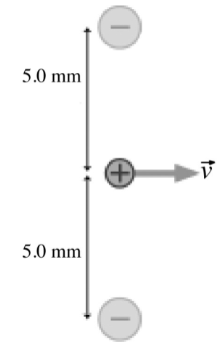
\includegraphics[scale=0.3]{figures/t5p7.png}
        \end{figure}
        \end{columns}
        
        \vspace{1em}
        
        ¿Cuál es la velocidad inicial mínima $v$ que necesita el protón para escapar totalmente de las cargas negativas?
        
        \begin{itemize}
        \item[A)] $1.8 \times 10^6$ m/s
        \item[B)] $3.5 \times 10^6$ m/s
        \item[C)] $6.8 \times 10^6$ m/s
        \item[D)] $1.4 \times 10^7$ m/s
        \end{itemize}
        
        \pause \centering \textbf{Respuesta:} A.
        
    \end{frame}

\begin{frame}{Semana 5 (05/03/2024) - T5P9}
    Una carga $Q$ se distribuye uniformemente en un anillo de radio $a$. Una carga puntual $q$ está fija en el centro del anillo, como se muestra en la figura. Un electrón es lanzado desde el infinito hacia el anillo a lo largo del eje del anillo. Este electrón se detiene momentáneamente en un punto del eje que está a una distancia $d$ del centro del anillo. ¿Cuál es la velocidad inicial del electrón en el infinito?
    
    \begin{figure}
        \centering
        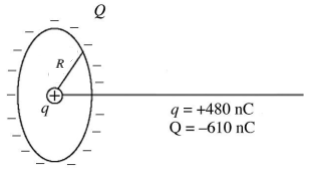
\includegraphics[scale=0.6]{figures/t5p9.png}
    \end{figure}
    
\end{frame}

\begin{frame}{Semana 5 (05/03/2024) - T5P10 (Bonus)}
    Two infinite plane sheets of surface charge, with densities $3\sigma_0$ and $-2\sigma_0$, are located a distance $\ell$ apart, parallel to one another. Discuss the electric field of this system. Now suppose the two planes, instead of being parallel, intersect at right angles. Show what the field is like in each of the four regions into which space is thereby divided.
\end{frame}

\begin{frame}{Semana 5 (05/03/2024) - T5P11}
    
Un cilindro sólido y muy largo, con radio $R$, tiene carga positiva distribuida de manera uniforme, con carga por unidad de volumen $\rho$.

\begin{itemize}
    \item[a)] Obtenga la expresión para el campo eléctrico dentro del volumen a una distancia $r$ del eje del cilindro en términos de la densidad de carga $r$.
    \item[b)] ¿Cuál es el campo eléctrico en un punto fuera del volumen en términos de la carga por unidad de longitud $l$ en el cilindro?
    \item[c)] Compare las respuestas de los incisos a) y  b) para $r = R$. 
    \item[d)] Elabore una gráfica de la magnitud del campo eléctrico como función de $r$, de $r = 0$ a $r = 3R$.
\end{itemize}

\end{frame}

\begin{frame}{Semana 5 (05/03/2024) - T5P11}
    \begin{itemize}
    
        \item[e)] A partir de la expresión para $E$ obtenida, obtenga las expresiones para el potencial eléctrico $V$ como
función de $r$, tanto dentro como fuera del cilindro. Sea $V = 0$ en la superficie del cilindro. En cada caso, exprese el resultado en términos de la
carga por unidad de longitud $l$ de la distribución de carga.
\item[f)] Elabore 
la gráfica de $V$ y $E$ como funciones de $r$, desde $r = 0$ hasta $r = 3R$.
    \end{itemize}
\end{frame}

\begin{frame}{Semana 6 (05/03/2024) - T5P12}

\small

Un cilindro metálico largo con
radio $a$ está apoyado en un soporte aislante sobre el eje de un tubo
metálico largo y hueco de radio $b$. La carga positiva por unidad de longitud del cilindro interior es igual a $\lambda$, y en el cilindro exterior hay una
carga negativa igual por unidad de longitud.
\begin{itemize}
    \item[a)] Calcule el potencial
$V(r)$ para \textbf{i.} $r < a$; \textbf{ii.} $a< r < b$; \textbf{iii.} $r > b$. (Sugerencia: El potencial neto
es la suma de los potenciales debidos a los conductores individuales).
Considere $V = 0$ en $r = b$.

\item[b)] Demuestre que el potencial del cilindro
interior con respecto al del exterior es

$$ V_{ab} = \frac{\lambda}{2\pi\epsilon_0} \ln\frac{b}{a}$$

\item[c)] Demuestre
que el campo eléctrico en cualquier punto entre los cilindros tiene una
magnitud igual a

$$ E = \frac{V_{ab}}{\ln(b/a)}\frac{1}{r} $$


\end{itemize}


\end{frame}

\begin{frame}{Semana 5 (05/03/2024) - T5P13}
    
     Una región en el espacio contiene una carga total
positiva $Q$ que está distribuida en forma esférica de manera que la densidad de carga volumétrica $\rho(r)$ está dada por

\begin{flalign*}
\rho(r) &=3\alpha r/(2R) \qquad \text{para }r\leq R/2, \\
\rho(r) &= \alpha\left[ 1-(r/R)^2 \right] \qquad \text{para }R/2\leq r\leq R, \\
\rho(r)&=0 \qquad \text{para }r\geq R.
\end{flalign*}

Aquí, $\alpha$ es una constante positiva que tiene unidades de C/m$^3$.

\begin{itemize}
    \item[a)] Determine $\alpha$ en términos de $Q$ y $R$.
    \item[b)] ¿Qué fracción de la carga
total está contenida
 dentro de la región $R/2 \leq r \leq R$?
\item[c)] ¿Cuál es la
magnitud de $\vec{E}$ en todos los puntos del espacio?
\item[d)] ¿Cuál es el valor del potencial eléctrico en todos los puntos del espacio?
\end{itemize}


\end{frame}

\begin{frame}{Semana 5 (05/03/2024) - T5P14}

En cierta región, existe una distribución de carga
con simetría esférica pero no uniforme. Es decir, la densidad de carga volumétrica $\rho(r)$ depende de la distancia $r$ del centro de la distribución, pero no de los ángulos polares esféricos $\theta$ y $\varphi$. El potencial eléctrico $V(r)$ debido a esta distribución de carga es $$
V(r)=\left\{\begin{matrix}
\frac{\rho_0a^2}{18\epsilon_0}\left[ 1-3\left(\frac{r}{a}\right)^2+2\left(\frac{r}{a}\right)^3 \right] & \text{para }r\leq a,
\\ 
0& \text{para }r\geq a
\end{matrix}\right.
$$
donde $\rho_0$ es una constante con unidades de $\text{C}/\text{m}^3$, y $a$ es una constante en metros. \begin{itemize}
    \item[a)] Obtenga expresiones de $\vec{E}$ para las regiones $r\leq a$ y $r\geq a$. Explique por qué $\vec{E}$ solo tiene una componente radial.
    
    \item[b)] Obtenga una expresión para $\rho(r)$ en cada una de las dos regiones $r\leq a$ y $r\geq a$. \textit{Sugerencia}: Utilice la ley de Gauss para dos cascarones esféricos, uno de radio $r$ y otro de radio $r+dr$. La carga contenida en el cascarón esférico infinitesimal de radio $dr$ es $dq = 4\pi r^2\rho(r)dr$.
\end{itemize}

\end{frame}

\begin{frame}{Semana 5 (05/03/2024) - T5P15}
    \small
    Un disco delgado con un agujero circular en el centro, llamado corona circular, tiene un radio interior $R_1$ y un radio exterior $R_2$ (\textit{ver} figura). El disco tiene una densidad de carga superficial uniforme y positiva $\sigma$ en su superficie.

\begin{itemize}
    \item[a)] Determine la carga
eléctrica total en la corona circular.
\item[b)] La corona circular se encuentra
en el plano $yz$, con su centro en el
origen. Para un punto arbitrario en
el eje $x$ (el eje de la corona circular), determine el potencial eléctrico.
\item[c)] Determine la magnitud y dirección del campo eléctrico para un punto arbitrario en
el eje $x$.

\begin{figure}[H]
        \centering
        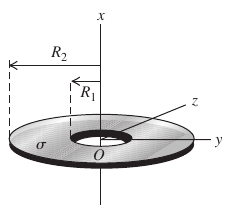
\includegraphics[scale=0.4]{figures/t5p15.png}
    \end{figure}

\end{itemize}
    
\end{frame}

\begin{frame}{Semana 5 (05/03/2024) - Q2}
    En la figura, un anillo de radio $R$ posee una carga $q$ distribuida uniformemente sobre él. Una carga puntual $Q$ es colocada en el centro del anillo. Determine la magnitud y el signo de $Q$ para que el campo eléctrico neto en un punto $P$ sobre el eje del anillo a una distancia $d$ de su centro sea cero. \\
    
    \begin{figure}[H]
        \centering
        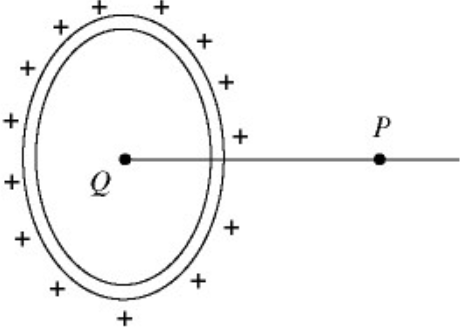
\includegraphics[scale=0.3]{figures/q2.png}
    \end{figure}
\end{frame}

\begin{frame}{Semana 6 (12/03/2023) - T6P1}
    Dos esferas huecas delgadas, conductoras y concéntricas están separadas por vacío. La esfera hueca interior tiene una carga total $+Q$ y radio $r_a$, y la esfera hueca exterior tiene carga $-Q$ y radio $r_b$. Determine la capacitancia de este capacitor esférico.
\end{frame}

\begin{frame}{Semana 6 (12/03/2023) - T6P2}
    Para el capacitor esférico descrito en el problema anterior, calcule la energía potencial eléctrica almacenada en el capacitor
    
    \begin{itemize}
        \item[a)] Usando la capacitancia $C$ obtenida
        \item[b)] Por integración de la densidad de energía $u$ del campo eléctrico.
    \end{itemize}
\end{frame}

\begin{frame}{Semana 6 (12/03/2023) - T6P3}
    %24.39
    El dieléctrico que ha de usarse en un capacitor de placas paralelas tiene una constante dieléctrica de 3.60 y rigidez dieléctrica de $1.60\times10^7 \text{ V}/\text{m}$. El capacitor debe tener una capacitancia de $1.25\times10^{-9} \text{ F}$ y debe soportar una diferencia de potencial máxima de 5500 V. ¿Cuál es el área mínima que deben tener las placas del capacitor?
    
\end{frame}

\begin{frame}{Semana 6 (12/03/2023) - T6P4}
    %34.66
    Un capacitor con aire está construido con dos placas planas, cada una con área $A$, separadas una distancia $d$. Después se inserta entre ellas un bloque metálico con espesor $a$ (menor que $d$) y de la misma forma y tamaño que las placas, paralelo a estas y sin tocarlas.

    \begin{figure}[H]
        \centering
        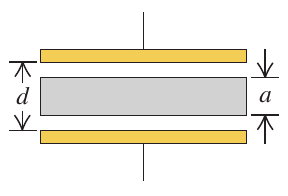
\includegraphics[scale=0.5]{figures/t6p4.png}
    \end{figure}
    
    \begin{itemize}
        \item[a)] ¿Cuál es la capacitancia de este arreglo?
        \item[b)] Exprese la capacitancia como un múltiplo de la capacitancia $C_0$ cuando el bloque de metal no está presente.
        \item[c)] Analice lo que ocurre con la capacitancia en los límites cuando $a\rightarrow0$ y $a\rightarrow d$.
    \end{itemize}
\end{frame}


\begin{frame}{Semana 6 (12/03/2023) - T6P5}
    Considere el siguiente arreglo de capacitores.
    
    \begin{figure}[H]
        \centering
        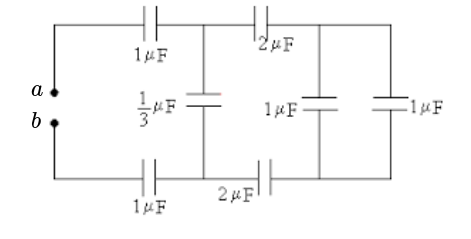
\includegraphics[scale=0.5]{figures/t6p5.png}
    \end{figure}
    
    La diferencia de potencial entre los puntos $a$ y $b$ es de 10 V. Determine:
    
    \begin{itemize}
        \item[a)] La capacitancia total del sistema
        \item[b)] La carga total que almacena el sistema.
        \item[c)] La energía total almacenada.
    \end{itemize}
\end{frame}

\begin{frame}{Semana 6 (12/03/2023) - T6P6}
    %24.60
    Los capacitores en la figura se encuentran inicialmente sin carga y están conectados, como se ilustra en el diagrama, con el interruptor $S$ abierto. La diferencia de potencial aplicada es $V_{ab} = +210 \text{ V}$.

    \begin{figure}[H]
        \centering
        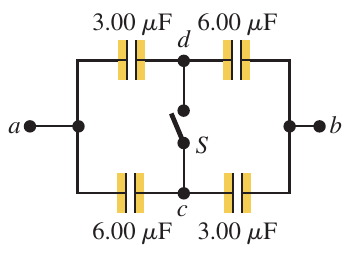
\includegraphics[scale=0.4]{figures/t6p6.png}
    \end{figure}
    
    \begin{itemize}
        \item[a)] ¿Cuál es la diferencia de potencial $V_{cd}$?
        \item[b)] ¿Cuál es la diferencia de potencial a través de cada capacitor una vez cerrado el interruptor $S$?
        \item[c)] ¿Cuánta carga fluyó a través del interruptor cuando se cerró?
    \end{itemize}
    
\end{frame}

\begin{frame}{Semana 6 (12/03/2023) - T6P7}
    Dos conductores cilíndricos delgados, coaxiales y largos están separados por un vacío. El cilindro interior tiene un radio $r_a$ y densidad de carga lineal $+\lambda$. El cilindro exterior tiene un radio $r_b$ y densidad de carga lineal $-\lambda$. Obtenga:
    
    \begin{itemize}
        \item[a)] La diferencia de potencial $V_{ab}$ entre ambos cilindros 
        \item[b)] La capacitancia por unidad de longitud
        \item[c)] La densidad de energía eléctrica del vacío entre cilindros $$u=\frac{1}{2}\epsilon_0 E^2$$
        \item[d)] La energía por unidad de longitud integrando la densidad de energía. Use $$U=\int u\, dV.$$ Considere $dV=2\pi Lr\,dr$.
    \end{itemize}
\end{frame}

\begin{frame}{Semana 7 (19/03/2023) - T7P1}

    El dieléctrico que ha de usarse en un capacitor de placas paralelas tiene una constante dieléctrica de 3.60 y rigidez dieléctrica de $1.60\times10^7 \text{ V}/\text{m}$. El capacitor debe tener una capacitancia de $1.25\times10^{-9} \text{ F}$ y debe soportar una diferencia de potencial máxima de 5500 V. ¿Cuál es el área mínima que deben tener las placas del capacitor?
\end{frame}

\begin{frame}{Semana 7 (19/03/2023) - T7P2}

    Dos placas conductoras cuadradas con lados de longitud $L$ están separadas por una distancia $D$. Se inserta un bloque dieléctrico con constante $K$ y dimensiones $L \times L \times D$, a una distancia $x$ en el espacio entre las placas, como se ilustra en la figura

    \begin{columns}
        \column{0.3\textwidth}
        \begin{figure}[H]
        \centering
        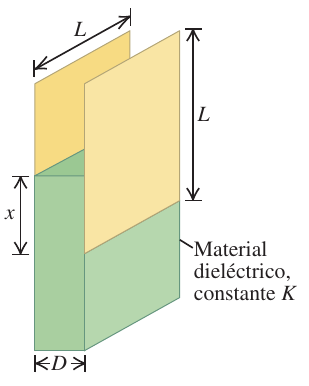
\includegraphics[scale=0.4]{figures/t7p2.png}
    \end{figure}
    \column{0.7\textwidth}
    \begin{itemize}
        \item[a)] Calcule la capacitancia $C$ de este sistema.
        \item[b)] Suponga que el capacitor está conectado a una batería que mantiene una diferencia de potencial constante $V$ entre las placas. Si el dieléctrico se inserta una distancia adicional $dx$ en el espacio entre las placas, demuestre que el cambio en la energía almacenada es $$dU=+\frac{(K-1)\epsilon_0V^2L}{2D}dx$$
    \end{itemize}
    \end{columns}
    
    
\end{frame}

\begin{frame}{Semana 7 (19/03/2023) - T7P3}
Un capacitor esférico aislado tiene carga $+Q$ en su conductor interior (radio $r_a$) y carga $-Q$ en su conductor exterior (radio $r_b$). Después, se llena la mitad del volumen entre los dos conductores con un líquido dieléctrico con constante $K$, como se muestra en el corte trans versal de la figura.

    \begin{columns}
        \column{0.3\textwidth}
        \begin{figure}[H]
        \centering
        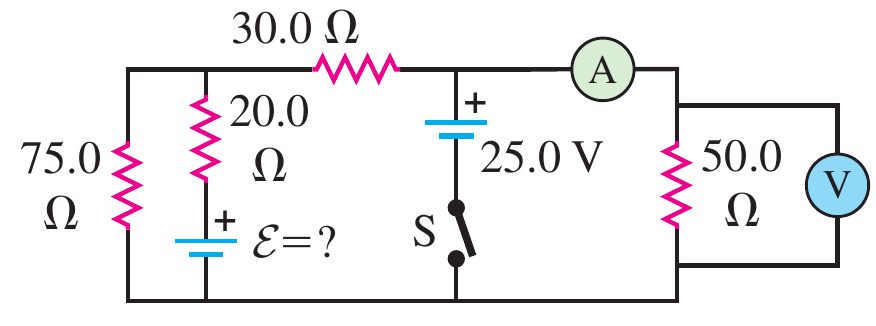
\includegraphics[scale=0.4]{figures/t7p3.png}
    \end{figure}
    \column{0.7\textwidth}
    \begin{itemize}
        \item[a)] Encuentre la capacitancia del capacitor medio lleno.
        \item[b)] Calcule la magnitud de $\vec{\boldsymbol{E}}$ en el volumen entre los dos conductores como función de la distancia $r$ desde el centro del capacitor. Dé respuestas para las mitades superior e inferior de este volumen.
    \end{itemize}
    \end{columns}

\end{frame}

\begin{frame}{Semana 7 (19/03/2023) - Q3}
La fórmula exacta para la capacitancia $C$ de un conductor en forma de esferoide alargado de longitud $2a$ y diámetro $2b$ es: $$C=\frac{8\pi\epsilon_0 a\epsilon}{\ln\left(\cfrac{1+\epsilon}{1-\epsilon}\right)},\qquad \text{donde} \qquad \epsilon=\sqrt{1-\frac{b^2}{a^2}}$$

\begin{itemize}
    \item[a)] Verifique que la fórmula se reduce a la expresión correcta para la capacitancia de una esfera si $b \rightarrow a$.
    \item[b)] Imagine que el esferoide es una gota de agua cargada. Si esta gota se deforma a volumen constante y carga constante $Q$ desde una esfera a un esferoide alargado, ¿aumentará o disminuirá la energía almacenada en el campo eléctrico? (El volumen de un esferoide es $\cfrac{4}{3}\pi ab^2$.)
\end{itemize}

\end{frame}

\begin{frame}{Semana 9 (02/04/2024) - T8P1}
    
    Dos bombillas tienen
resistencias de $400$ y $800$ $\Omega$. Si están conectadas en serie a través 
de una línea de 120 V, calcule 
    
    \begin{itemize}
        \item[a)] La corriente que pasa por cada bombilla.
        \item[b)] La potencia disipada por cada una.
        \item[c)] La potencia total disipada
en ambas bombillas.
    \end{itemize}

    Ahora, las bombillas se conectan en paralelo a
través de la línea de 120 V. Obtenga

    \begin{itemize}
        \item[d)] La corriente a través de cada
bombilla.
        \item[e)] La potencia disipada en cada bombilla.
        \item[f)] La potencia total
que se disipa en las dos bombillas.
        \item[g)] En cada situación, ¿cuál es la
bombilla más luminosa?
        \item[h)] ¿En cuál situación hay una salida total
mayor de luz de ambas bombillas combinadas?
    \end{itemize}
    
\end{frame}

\begin{frame}{Semana 9 (02/04/2024) - T8P2}

Para el circuito que se presenta en la figura, los dos medidores son ideales, la batería no tiene resistencia interna apreciable y el
amperímetro da una lectura de 1.25 A.

\begin{figure}
    \centering
    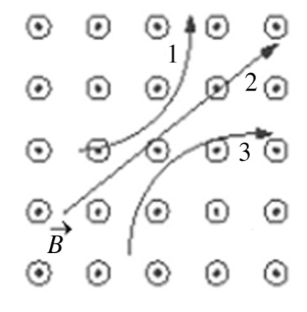
\includegraphics[scale=0.2]{figures/t8p2.png}
\end{figure}

\begin{itemize}
    \item[a)] ¿Cuál es la lectura del voltímetro?
    \item[b)] ¿Cuál es la fem $\mathcal{E}$ de la batería?
    
\end{itemize}
    
\end{frame}

\begin{frame}{Semana 9 (02/04/2024) - T8P3}
    
    En el circuito que se presenta en la figura, las baterías tienen resistencias internas despreciables y los dos medidores son ideales. Con el interruptor $S$ abierto, el voltímetro da una lectura de 15.0 V.
    
    \begin{figure}
    \centering
    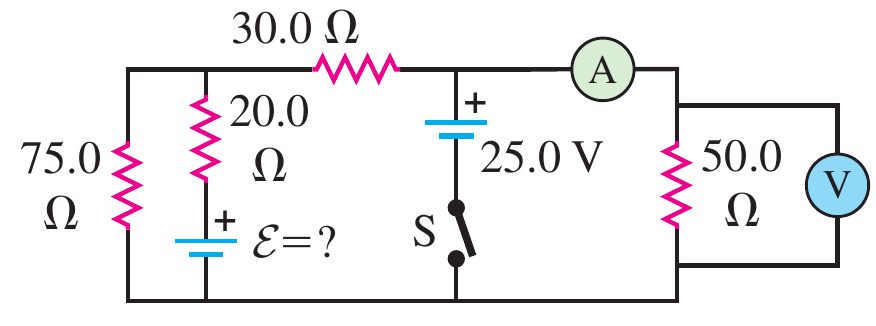
\includegraphics[scale=0.2]{figures/t8p3.png}
    \end{figure}
    
    \begin{itemize}
        \item[a)] Calcule la fem $\mathcal{E}$ de la batería.
        \item[b)] ¿Cuál será la lectura del amperímetro cuando se cierre el interruptor?
    \end{itemize}
    
\end{frame}

\begin{frame}{Semana 9 (02/04/2024) - T8P4}

    \begin{itemize}
        \item[a)] En la figura, ¿cuál es el potencial del punto $a$ con respecto al punto $b$
cuando el interruptor $S$ está abierto?
        \item[b)] ¿Cuál punto, $a$ o $b$, está a un mayor
potencial?
        \item[c)] ¿Cuál es el potencial final
del punto $b$ con respecto a tierra cuando
el interruptor $S$ está cerrado?
        \item[d)] ¿Cuánto cambia la carga en cada capacitor
cuando S está cerrado?
    \end{itemize}

    \begin{figure}
    \centering
    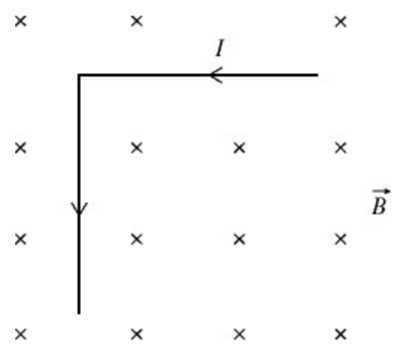
\includegraphics[scale=0.6]{figures/t8p4.png}
    \end{figure}

    
\end{frame}

\begin{frame}{Semana 9 (02/04/2024) - T8P5}
    
    Como se muestra en la figura, una red de resistores de resistencias $R_1$ y $R_2$ se extiende infinitamente hacia la derecha.
    
    \begin{figure}
    \centering
    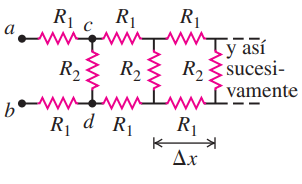
\includegraphics[scale=0.6]{figures/t8p5.png}
    \end{figure}
    
    Demuestre que la resistencia total $R_T$ de la red infinita es igual a

    \begin{equation}
        R_T=R_1+\sqrt{R_1^2+2R_1R_2}
    \end{equation}
    
    (\textit{Sugerencia}: como la red es infinita, su resistencia a la derecha de los puntos $c$ y $d$ también es igual a $R_T$.)
    
\end{frame}

\begin{frame}{Semana 9 (02/04/2024) - T8P6}
    
    A multiloop circuit is shown in the figure. It is not necessary to solve the entire circuit. The current $I_2$ is closest to

    \begin{figure}
    \centering
    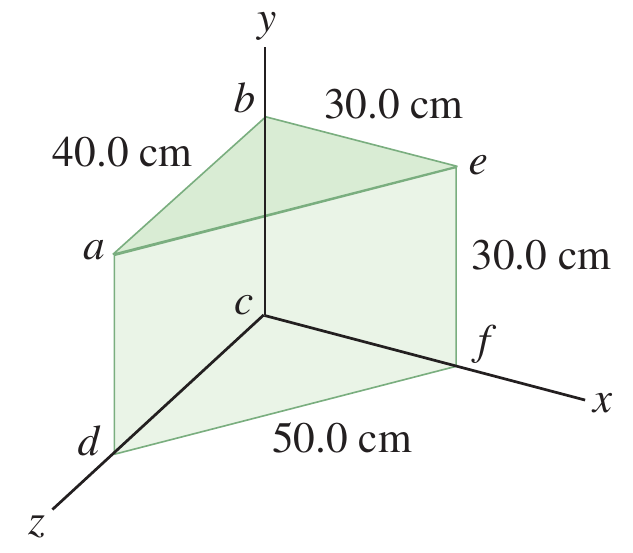
\includegraphics[width=0.5\textwidth]{figures/t8p6.png}
    \end{figure}
    
\end{frame}

\begin{frame}{Semana 10 (09/04/2024) - T9P1}

    An electron moving in the direction of the $+x$-axis enters a magnetic field. If the electron experiences a magnetic deflection in the $-y$ direction, the direction of the magnetic field in this region points in the direction of the
   
   \begin{itemize}
       \item[A)] $+z$-axis.
       \item[B)] $-z$-axis.
       \item[C)] $-z$-axis.
       \item[D)] $+y$-axis.
       \item[E)] $-y$-axis.
   \end{itemize}
   
   \pause \centering \textbf{Answer:} B.
    
\end{frame}

\begin{frame}{Semana 10 (09/04/2024) - T9P2}
    
    Three particles travel through a region of space where the magnetic field is out of the page, as shown in the figure.
    
    \begin{columns}
        \column{0.5\textwidth}
        \begin{figure}
        \centering
        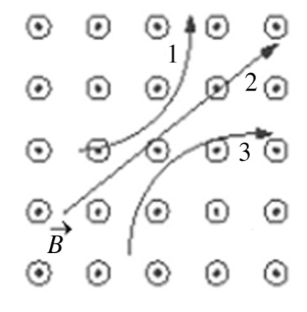
\includegraphics[scale=0.3]{figures/t9p2.png}
    \end{figure}
    
    The electric charge of each of the three particles is, respectively
    \column{0.5\textwidth}
    \begin{itemize}
       \item[A)] 1 is neutral, 2 is negative, and 3 is positive.
       \item[B)] 1 is neutral, 2 is positive, and 3 is negative.
       \item[C)] 1 is positive, 2 is neutral, and 3 is negative.
       \item[D)] 1 is positive, 2 is negative, and 3 is neutral.
       \item[E)] 1 is negative, 2 is neutral, and 3 is positive.
   \end{itemize}
    \end{columns}
    \pause \centering \textbf{Answer:} E.
    
\end{frame}

\begin{frame}{Semana 10 (09/04/2024) - T9P3}
    
    A charge is accelerated from rest through a potential difference $V$ and then enters a uniform magnetic field oriented perpendicular to its path. The field deflects the particle into a circular arc of radius $R$. If the accelerating potential is tripled to $3V$, what will be the radius of the circular arc?
    
    \begin{itemize}
       \item[A)] $9R$.
       \item[B)] $3R$.
       \item[C)] $\sqrt{3}R$.
       \item[D)] $R/\sqrt{3}$.
       \item[E)] $R/9$.
   \end{itemize}
    
    \pause \centering \textbf{Answer:} C.
    
\end{frame}

\begin{frame}{Semana 10 (09/04/2024) - T9P4}
    
    Una partícula con carga de $-1.24 \times10^{-8}$ C se mueve con
velocidad instantánea $\vec{v}= (4.19 \times 10^4 \text{ m/s})\hat{\imath} + (-3.85 \times 10^4 \text{ m/s})\hat{\jmath}$.
Determine la fuerza que sobre esta partícula ejerce un campo magnético de:
\begin{itemize}
    \item[a)] $\vec{B} = (1.40 \text{ T})\hat{\imath}$
    \item[b)] $\vec{B} = (1.40 \text{ T})\hat{k}$
\end{itemize}
    
\end{frame}

\begin{frame}{Semana 10 (09/04/2024) - T9P5}
    Una partícula con carga de $-5.60$ nC se mueve en un
campo magnético uniforme $\vec{B}=-(1.25 \text{ T})\hat{k}$ . La medición de la fuerza magnética sobre la partícula resulta ser $\vec{F}=(3.40 \times 10^{-7} \text{ N})\hat{\imath} + (7.40 \times 10^{-7} \text{ N})\hat{\jmath}$.

\begin{itemize}
    \item[a)] Calcule todas las componentes que pueda de la velocidad de la partícula con base en esta información.
    \item[b)] ¿Hay componentes de la velocidad que no estén determinadas por la medición 
de la fuerza? Explique su respuesta.
    \item[c)] Calcule el producto escalar $\vec{v}\cdot\vec{F}$ y diga cuál es el ángulo entre $\vec{v}$ y $\vec{F}$.
\end{itemize}
\end{frame}

\begin{frame}{Semana 10 (09/04/2024) - T9P6}
    Un grupo de partículas se mueve en un campo magnético de magnitud y dirección desconocidas. Usted observa que un protón
que se mueve a $1.50$ km/s en la dirección $+x$ experimenta una fuerza
de $2.25 \times 10^{-16}$ N en la dirección $+y$, y otro electrón que se mueve a
4.75 km/s en la dirección $-y$ experimenta una fuerza de $8.50 \times 10^{-16}$ N
en la dirección $-x$.
\begin{itemize}
    \item[a)] ¿Cuáles son la magnitud y la dirección del
campo magnético?
    \item[b)] ¿Cuáles son la magnitud y la dirección de la
fuerza magnética sobre un electrón que se mueve en la dirección $-x$
a 3.20 km/s?
\end{itemize}
\end{frame}

\begin{frame}{Semana 10 (09/04/2024) - T9P7}
    El campo magnético en cierta región es de 0.128 T, y su
dirección es la del eje $+z$ en la
figura.

\begin{figure}
    \centering
    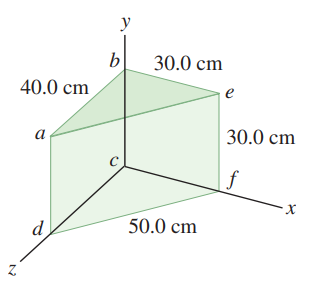
\includegraphics[width=0.3\textwidth]{figures/t9p7.png}
\end{figure}

\begin{itemize}
    \item[a)] ¿Cuál es el flujo
magnético a través de la superficie
$abcd$ en la figura?
    \item[b)] ¿Cuál es el
flujo magnético a través de la
superficie $befc$?
    \item[c)] ¿Cuál es el flujo
magnético a través de la superficie
$aefd$?
    \item[d)] ¿Cuál es el flujo neto a
través de las cinco superficies que
encierran el volumen sombreado?
\end{itemize}
\end{frame}

\begin{frame}{Semana 10 (09/04/2024) - T9P8}
    
     Considere un protón ($q=1.60\times10^{-19}$ C, $m= 1.67\times 10^{-27}$ kg) que se mueve en un campo magnético uniforme $\vec{B}=(0.500\text{ T})\hat{i}$. En $t=0$ el protón tiene componentes de velocidad $v_x=1.50\times10^5$ m/s, $v_y=0$ y $v_z=2.00\times10^5$ m/s

\begin{itemize}
    \item[a)] ¿Cuáles son la magnitud y dirección de la fuerza magnética que actúa sobre el protón? 
    
    \end{itemize}
    
    Además del campo magnético, hay un campo eléctrico uniforme $\vec{E}=(+2.00\times 10^4\text{ V/m)}\hat{i}$.
    
    \begin{itemize}
    \item[b)] ¿El protón tendrá una componente de aceleración en la dirección del campo el\'ectrico?
    \item[c)] Describa la trayectoria del prot\'on. ¿El campo el\'ectrico afecta el radio de la hélice? Explique su respuesta.
    
    \item[d)] En $t=T/2$, donde $T$ es el periodo del movimiento circular del protón, ¿cuál es la componente $x$ del desplazamiento del protón a partir de su posición en $t=0$?

\end{itemize}

    
\end{frame}

\begin{frame}{Semana 10 (09/04/2024) - T9P9}
    Una partícula de carga $q>0$ se mueve con rapidez $v$ en la
dirección $+z$ a través de una región de campo magnético uniforme.
La fuerza magnética sobre la partícula es $\vec{F}=F_0(3\hat{\imath}+4\hat{\jmath})$, donde $F_0$
es una constante positiva.
\begin{itemize}
    \item[a)] Determine las componentes $B_x$, $B_y$ y $B_z$,
o las que sean posibles con la información proporcionada.
    \item[b)] Si además se tiene el dato de que la magnitud del campo magnético es de
$6F_0/(qv)$, determine tantas de las componentes restantes de como sea
posible.
\end{itemize}
\end{frame}

\begin{frame}{Semana 10 (09/04/2024) - Q4}

¿Cuál es la diferencia de potencial entre los puntos $a$ y $b$ en el circuito que se muestra en la figura?

\begin{figure}[H]
        \centering
        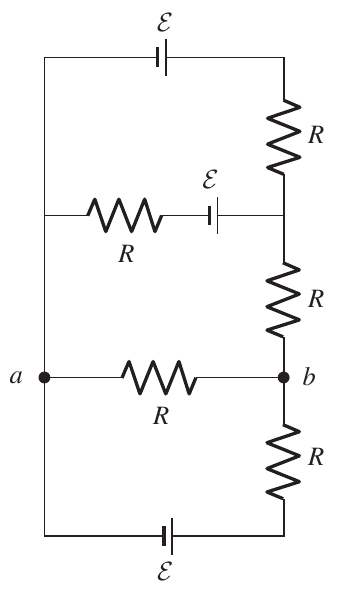
\includegraphics[scale=0.3]{figures/q4.png}
    \end{figure}
    
\end{frame}